\documentclass[12pt]{article}
\usepackage[utf8]{inputenc}
\usepackage{acronym}
\usepackage{amsmath}
\usepackage{amsfonts}
\usepackage{amssymb}
\usepackage{booktabs}
\usepackage{braket}
\usepackage{changepage}
\usepackage{enumitem}
\usepackage{fancyhdr}
\usepackage{graphicx}
\usepackage{geometry}
\usepackage[none]{hyphenat}
\usepackage{lipsum}
\usepackage{multicol}
\usepackage[numbers]{natbib}
\usepackage{parskip}
\usepackage{subcaption}
\usepackage{tabularx}
\geometry{a4paper, margin=1in}
\setlength{\columnsep}{0.7cm}
\newcommand{\vctr}[1]{\ensuremath{\mathbf{#1}}}
\newcommand{\vctrg}[1]{\mbox{\boldmath{$#1$}}}
\newcommand{\unitr}[1]{\ensuremath{\mathbf{\hat{#1}}}}
\newcommand{\depar}[2]{\ensuremath{\frac{\partial#1}{\partial#2}}}
\newcommand{\depars}[2]{\ensuremath{\frac{\partial^{2}#1}{\partial#2^{2}}}}
\newcommand{\perme}{\ensuremath{\epsilon_{0}}}
\newcommand{\permm}{\ensuremath{\mu_{0}}}
\newcommand{\unitrg}[1]{\mbox{\boldmath{$\hat{#1}$}}}

\title{Bruce A Nuclear Generation Station (BANGS) Cooling System}
\author{Md. Ariful Islam \\ Email: islamm65@mcmaster.ca \\ Department of Engineering Physics, McMaster University}
\date{}     

\begin{document}

% Header & Footer Stuff
\pagestyle{fancy}
\fancyhf{}                       % Clear default headers and footers
\fancyhead[L]{Bruce (BANGS) Cooling System} 
\fancyhead[R]{\today}           
\renewcommand{\headrulewidth}{0.4pt} 
\fancyfoot[C]{\thepage}

\maketitle
\thispagestyle{fancy}

\section*{\centering Abstract} 

\begin{adjustwidth}{0.5in}{0.5in}

\textit{The thermal-hydraulic design of Bruce A Nuclear Generating Station ensures efficient heat removal and reactor stability under various operating conditions. This assignment examines key thermal-hydraulic aspects, including heat transport, shutdown cooling, pressure control, and transient responses. The primary heat transport (HT) system, which uses heavy water as coolant, operates under high pressure conditions to transfer heat from the reactor core to the steam generators. Various scenarios, such as total loss of Class IV power, partial HT pump failures, and loss-of-coolant accidents (LOCA), are analyzed to assess the plant response mechanisms. Reactor trip functions, stepback signals, and multiple cooling systems ensure safety and operational continuity. The study highlights the robust design of the plant and its redundancy in heat removal systems, reinforcing its ability to effectively manage normal and abnormal conditions.}
\end{adjustwidth}

%% -----------------------
%%      Introduction
%% -----------------------
\begin{multicols}{2}

\section{Inroduction}

Bruce A is a four-unit nuclear generating station located in the northwest corner of the Bruce Power site, approximately 2.5 km northeast of Douglas Point, Ontario \cite{BruceSafetyReport2006}. The station comprises Units 1, 2, 3, and 4 and is operated by Bruce Power A L.P. Originally designed by Atomic Energy of Canada Limited (AECL) and Ontario Hydro (OH), Bruce A was initially operated by Ontario Hydro before transitioning to Bruce Power. The four units were brought into service between 1976 and 1978, marking a significant milestone in Canada’s nuclear energy sector. Following refurbishment plans, Unit 4 was returned to service in October 2003, followed by Unit 3 in January 2004, and Units 1 and 2 are brought back into service in 2012. The Bruce A facility, like its counterpart Bruce B, utilizes CANDU (CANada Deuterium Uranium) technology, which relies on pressurized heavy water for neutron moderation and cooling.

The key specifications of Bruce A are as follows:

\begin{itemize}
    \item \textbf{Core thermal power:} 2,832 MW(th) per unit.
    \item \textbf{Gross electrical maximum continuous rating:} 825 MW(e) per unit.
    \item \textbf{Net electrical maximum continuous rating:} 769 MW(e) per unit.
    \item \textbf{Total nominal net station output:} 3,392 MW(e) across four units.
    \item \textbf{Reactor type:} CANDU pressurized heavy water reactor designed by AECL and Ontario Hydro.
    \item \textbf{Containment:}  Reinforced concrete structure designed by Ontario Hydro.

\end{itemize}

To compare the main design parameters between Bruce A and Bruce B, the Table \ref{tab:tab_1} summarizes key thermal-hydraulic characteristics.

Each Bruce A reactor consists of a horizontal, cylindrical calandria with integral endshields, fuel channel assemblies, and reactivity control mechanisms (Figure \ref{fig:fig_1}). The reactor core is enclosed within a shield tank filled with light water, which serves as biological shielding. The calandria, which contains heavy water $(D_{2}O)$ as both a moderator and reflector, is penetrated by 480 calandria tubes, housing the fuel channel assemblies. This multi-compartment structure, which includes the endshields and shield tank, provides both operational shielding and full shutdown shielding between the calandria and the reactor vault.

The Heat Transport (HT) system is responsible for extracting heat from the reactor core. It circulates pressurized heavy water through the fuel channels, removing the heat generated by nuclear fission. This heat is subsequently transferred to light water in the steam generators, where it produces steam to drive turbines for electricity generation. The HT system consists of:
\begin{itemize}
    \item \textbf{Four primary circulating pumps} that drive the coolant flow.
    \item \textbf{Six headers} that distribute the coolant.
    \item \textbf{Feeder pipes} that connect the fuel channels to the headers.
    \item \textbf{Eight steam generators} that facilitate heat exchange.
    \item \textbf{Four preheaters.}
    \item A \textbf{pressurizer} connected to the east outlet header, which regulates system pressure through a combination of steam bleed valves and immersion heaters.
\end{itemize}

\end{multicols}

\begin{table}
    \centering
\caption{Main Design Parameters and Features}
\label{tab:tab_1}
    \begin{tabular}{ccc} 
    \hline
    Parameter & Bruce A  & Bruce B \\ 
    \hline
    No. of HT Loops & 1  & 1 \\ 
    No. of Zones & 2 & 2 \\ 
    ROH (Reactor Outlet Header) Pressure (MPa) & 9.18 & 9.31 \\ 
    ROH Temperature $^{\circ}$F & 579 & 579 \\ 
    RIH (Reactor Inlet Header) Temperature $^{\circ}$F & 483 & 483\\ 
    Maximum Channel Flow (lbm/hr) & 190000 & 190000\\ 
    No. of Fuel Channels & 480 & 480\\ 
    No. of Circulating Pumps & 4 & 4\\ 
    No. of Steam Generators & 8 & 8\\ 
    No. of Preheaters & 4 & 4 \\ 
    Power Output (MW) & 750 & 750 \\ 
    Pressurizer Volume $(ft^3)$ & 1200 & 1200 \\ 
    \hline
         
    \end{tabular}
    
\end{table}

\begin{figure}
    \centering
    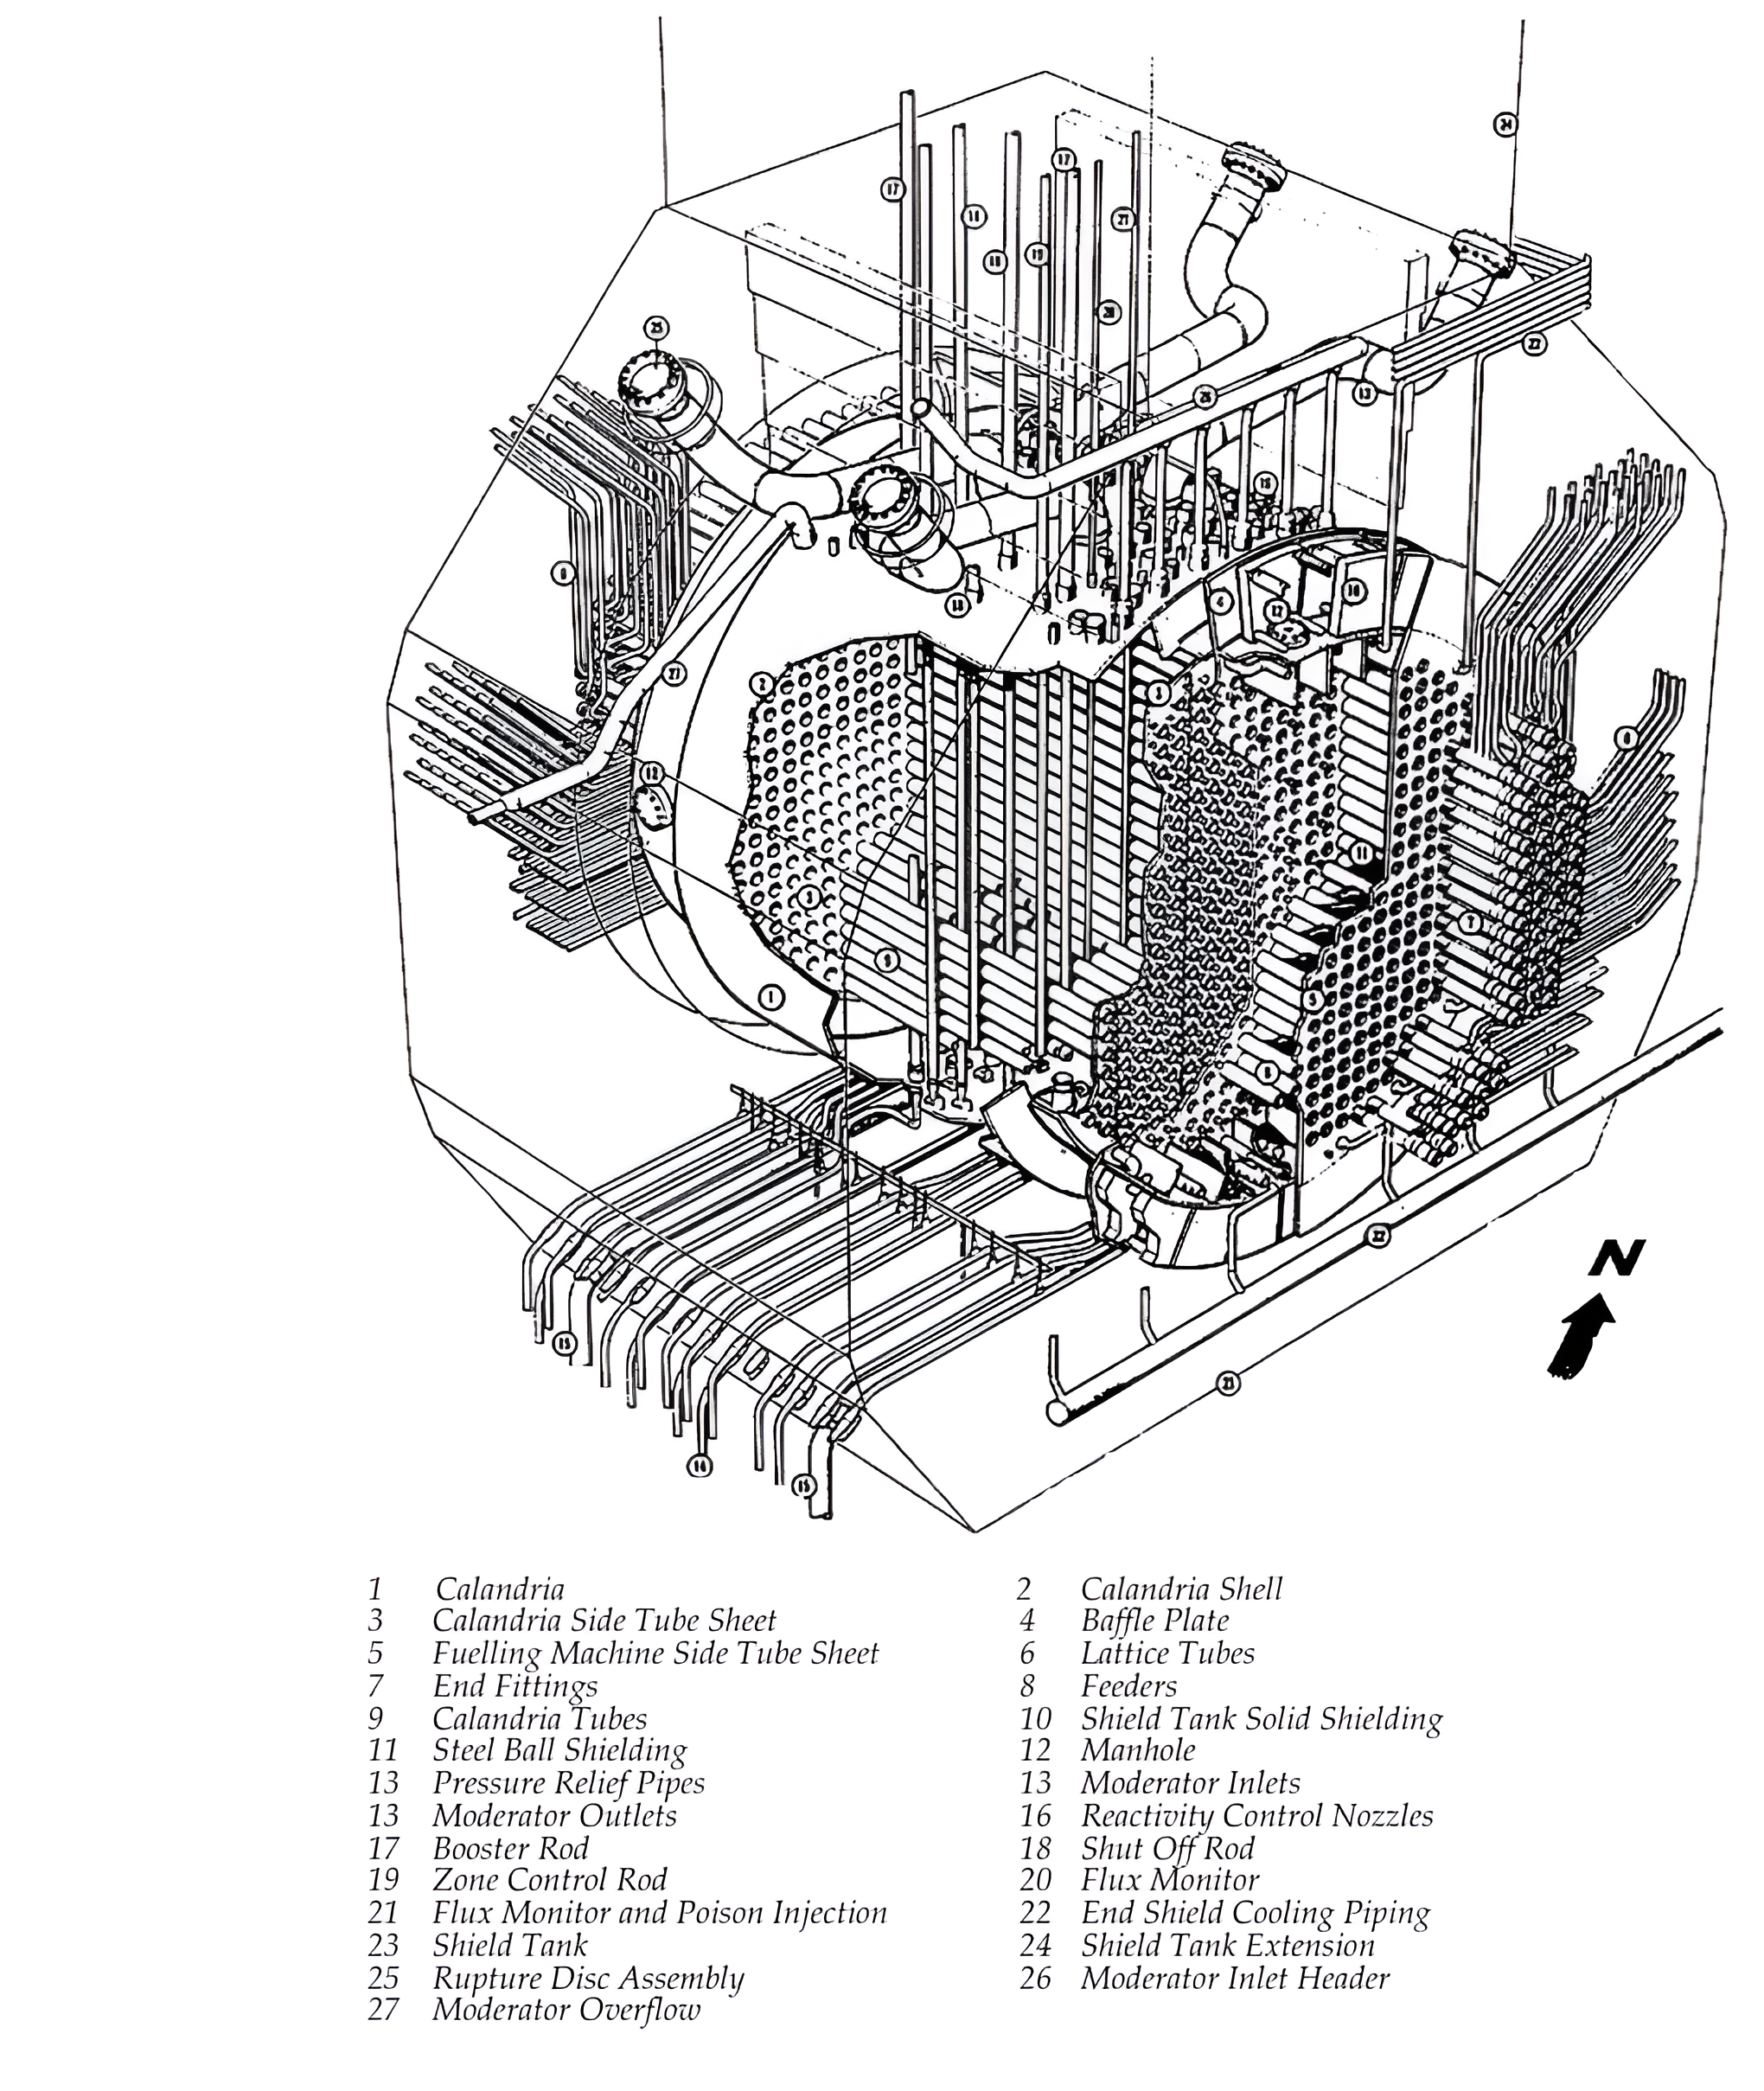
\includegraphics[width=0.6\linewidth]{figs/bruce_a.png}
    \caption{Reactor Assembly Bruce A}
    \label{fig:fig_1}
\end{figure}

%% -----------------------------------
%%      Cooling System Overview
%% ----------------------------------

\begin{multicols}{2}
\section{BANGS Cooling System Overview}

The Bruce A reactor unit features a single-loop heat transport system, as shown in Figure \ref{fig:fig_2}. This system consists of four circulating pumps, eight steam generators, and four external pre-heaters. The two-zone coolant configuration in Bruce A was designed to enhance heat removal in high-power fuel channels without inducing boiling, increasing system pressure, or significantly altering channel flow or boiler area.

The 280 channels in the inner zone generate more power than the 200 channels in the outer zone. To accommodate this, the heat transport system employs a sub-cooled heavy water $(D_{2}O)$ coolant flow. Coolant entering the inner zone is pre-cooled by pre-heaters. The outer zone bypass flow, which skips the preheater, enters at a higher temperature (510$^{\circ}$F) compared to the preheater outlet flow (484$^{\circ}$F). The inner zone receives coolant from the preheater flow, while the outer zone receives the bypass flow. Despite these variations, all channels operate with an approximately uniform outlet temperature of 581$^{\circ}$F (305$^{\circ}$C) and discharge into a single outlet header on each side of the reactor.

The key thermal-hydraulic parameters at critical locations are:

\begin{itemize}
    \item \textbf{Outlet header pressure:} 9.18 MPa
    \item \textbf{Inlet header pressure:} 11.25 MPa
    \item \textbf{Total coolant mass flow rate:} $2.25 \times 10^7$ lb/h
    \item \textbf{Bypass inlet channel mass flow rate:} $1.3 \times 10^7$ lb/hr
\end{itemize}

The channel velocity is limited to $10\ m/s$ due to fretting considerations of the fuel bundle and pressure tube. The pressurizer is connected to the main heat transport system at one of the steam generator inlet lines by the pressurizer connection line. A valve is provided to isolate the pressurizer from the heat transport system during maintenance shutdowns. Temperature Distribution of Fuel and Structural Components are:

\begin{itemize}
    \item \textbf{Fuel Centerline Temperature:} Peaks at approximately 2500$^{\circ}$F (1370$^{\circ}$C) under nominal full-power conditions.
    \item \textbf{Cladding Surface Temperature:} Typically around 600–700$^{\circ}$F (315–370$^{\circ}$C), depending on local power levels and heat transfer efficiency.
    \item \textbf{Pressure Tube Temperature:} The external surface temperature ranges between 570–590$^{\circ}$F (300–310$^{\circ}$C), while the inner surface (facing the coolant) is slightly cooler due to direct heat transfer from the coolant.
    \item \textbf{Calandria Tube Temperature:} Approximately 250–300$^{\circ}$F (120–150$^{\circ}$C).
\end{itemize}

\end{multicols}

\begin{figure}
    \centering
    \includegraphics[width=0.7\linewidth]{figs/HTS.png}
    \caption{Heat Transport System (Bruce A)}
    \label{fig:fig_2}
\end{figure}

%% -----------------------------------
%%      Key components
%% ----------------------------------
\begin{multicols}{2}

\section{Design of Key \\ Components in the \\ Primary Heat \\  Transport System}
\subsection{Steam Generators}

The steam generators (SGs) in Bruce A play a crucial role in transferring heat from the heavy water $(D_{2}O)$ coolant in the primary heat transport system to light water in the secondary side, generating steam to drive the turbine. Each SG consists of an inverted U-tube bundle housed within a cylindrical shell. The primary side of each SG comprises the SG head, the tube bundle, and the primary side of the tube sheet. A divider plate inside the SG head separates the inlet and outlet halves, directing the coolant flow through the tube bundle. The Incoloy U-tubes are welded and rolled into an Inconel-clad carbon steel tube sheet, ensuring high resistance to corrosion and thermal stresses. At full power, $(D_{2}O)$ coolant enters the SG, as it flows through the tubes, the coolant condenses and cools before returning to the reactor inlet header. A key difference between the Bruce A and Pickering SGs is the separate feedwater preheaters. In Bruce A, a portion of the primary coolant is diverted through these preheaters. This extracted heat is utilized to raise the temperature of the boiler feedwater. The key parameters of the steam generators for Bruce A unit are summarized in Table \ref{tab:tab_2}.
    
\end{multicols}

\begin{table}[h]
    \centering
    \caption{Key Parameters of Bruce A Steam Generators \cite{tapping2000candu}}
    \label{tab:tab_2}
    \renewcommand{\arraystretch}{1.2}
    \begin{tabularx}{\textwidth}{X X} % Auto-adjusts column width
    \hline
    \textbf{Parameter} & \textbf{Value} \\ 
    \hline
    Number of tubes per SG & 4200  \\ 
    Thermal output per SG $(MW_{th})$ & 280 \\ 
    Tube material & Inconel 600 \\ 
    Tube outer diameter (OD) & 12.7 mm \\ 
    Primary coolant temperatures $(T_{hot} / T_{cold})$ & 304$^{\circ}$C / 265$^{\circ}$C \\ 
    Secondary steam temperature & 256$^{\circ}$C \\ 
    Tube supports & Carbon steel trifoil broached tube support plates (TSP) \\ 
    U-bend supports & Stacked carbon steel scallop bars \\ 
    Preheater configuration & Separate \\ 
    Condenser cooling water source & Lake Huron \\ 
    \hline
    \end{tabularx}
\end{table}

\begin{multicols}{2}
    \subsection{Heat Transport Pumps}

    The heat transport pumps in Bruce A are vertical, single-stage, single-suction, centrifugal pumps with a volute-type casing \cite{pon_2024_my8h2-66b34}. Each pump features a radial guide bearing, lubricated by the pumped heavy water $(D_{2}O)$, and a tilting pad-type guide bearing with a double-acting thrust bearing in the motor. The pump shaft is sealed using mechanical shaft seals to prevent leakage. Each pump is driven by a vertically mounted, totally enclosed, air-water cooled, squirrel cage induction motor. A solid flywheel is integrated into the motor to improve stability. A typical Bruce A heat transport pump is shown in Figure \ref{fig:fig_3}, and its key characteristics are summarized in Table \ref{tab:tab_3}.
    
\end{multicols}

\begin{figure}
    \centering
    \includegraphics[width=0.5\linewidth]{figs/pumps.png}
    \caption{Primary Heat Transport Pump}
    \label{fig:fig_3}
\end{figure}

\begin{table}[h]
    \centering
    \caption{Key Parameters of Bruce A Heat Transport Pumps}
    \label{tab:tab_3}
    \renewcommand{\arraystretch}{1.2}
    \begin{tabularx}{\textwidth}{X X} % Auto-adjusts column width
    \hline
    \textbf{Parameter} & \textbf{Value} \\ 
    \hline
    Pump type & Vertical, Centrifugal, Single-stage  \\ 
    Flow rate & 3.307 $m^3/s$ \\ 
    Discharge pressure/temperature & 10.625 MPa / 265$^{\circ}$C \\ 
    Operating speed & 1800 rpm \\ 
    Flywheel & Solid (integrated in motor) \\ 
    Pump bearings & Hydrostatic, $(D_{2}O)$-energized \\
    \hline
    \end{tabularx}
\end{table}

\begin{multicols}{2}

\subsection{Feeders, Headers and HTS Piping}

The feeder/header and end fitting arrangements are shown in Figure \ref{fig:fig_4}. In Bruce A unit, the Primary Heat Transport (PHT) system consists of 480 inlet feeder pipes and 480 outlet feeder pipes connecting to multiple headers (4 inlet headers and 2 outlet headers), with each reactor having a total of 960 feeder pipes in total. An inlet and an outlet feeder connect each fuel channel to the large diameter HTS piping system. Each feeder consists of a single small diameter (38 mm to 88 mm dia.) pipe run starting with a mechanical connection at the fuel channel and ending at the welded connection at the header nozzle. Due to the fuel channel arrangement, the feeders are grouped in arrays of small diameter pipes following essentially parallel paths from the reactor face to the headers. Feeder lengths vary from 6 to 20 meters. The feeders are enclosed in an insulated feeder cabinet and experience hot dry atmosphere during reactor operation. Carbon steel piping is used to minimize the possibility of chemically induced stress corrosion cracking.

\end{multicols}

\begin{figure}
    \centering
    \includegraphics[width=0.5\linewidth]{figs/feeder-header.png}
    \caption{Feeder and Header Arrangement}
    \label{fig:fig_4}
\end{figure}

\begin{multicols}{2}

\subsection{Auxiliary Systems}

The Heat Transport (HT) system interconnects with several auxiliary systems, including Pressure and Inventory Control System, $D_2O$ Collection System, the Shutdown Cooling System and the Purification System. These systems support reactor operation by maintaining coolant inventory, pressure regulation, purification, and cooling during shutdown.

\subsubsection{Pressure and Inventory Control System}

The HT pressure and inventory control system consists of: pressurizer, a feed pump, a storage tank and feed and bleed valves. Its primary functions are to:

\begin{itemize}
    \item Maintain pressure and inventory control for each heat transport circuit.
    \item Provide overpressure protection.
    \item Regulate controlled degassing flow.
\end{itemize}

During normal operation at full power, the pressurizer controls system pressure, while the feed and bleed circuit maintains coolant inventory. At low reactor power ($<5\%$) or during shutdown, the pressurizer is isolated, and pressure control is managed solely by the feed and bleed circuit, a state referred to as ‘solid mode’ operation.

\subsubsection{$D_{2}O$ Collection System}

The $D_{2}O$ collection system is responsible for:
\begin{itemize}
    \item Collecting drainage from equipment before maintenance.
    \item Recovering leakage from mechanical components.
    \item Receiving $D_{2}O$ sampling flow.
\end{itemize}

If the isotopic purity of the collected $D_{2}O$ meets the required standard, it is pumped to storage tanks for reuse in the HT system.

\subsubsection{Shutdown Cooling System}

The shutdown cooling system consists of a pump and heat exchanger at each end of the reactor connected between the outlet and inlet headers of each loop of the heat transport system. Its key functions include:
\begin{itemize}
    \item Cooling the heat transport system from 177$^{\circ}$C to 54$^{\circ}$C, where it can be maintained indefinitely.
    \item Providing core cooling during maintenance of steam generators and heat transport pumps.
    \item Maintaining header levels during maintenance operations.
\end{itemize}

\subsubsection{Purification System}

The purification system operates using flow provided by the HT pumps and serves to:
\begin{itemize}
    \item Limit corrosion product accumulation by removing soluble and insoluble impurities.
    \item Remove fine solid accumulations that may be released due to chemical, hydraulic, or thermal transients.
    \item Minimize radioactive contamination within the HT system.
    \item Maintain pH and isotopic purity of the $D_2O$ coolant.
\end{itemize}

\subsubsection{Emergency Core Cooling System}

This is one of the major safety systems. The heat transport system is an integral part of the emergency core cooling system. Its function is to provide cooling water to the reactor core following a loss of coolant accident (LOCA). The objective is to limit damage to the fuel and limit the release of radioactive materials from the station so that the applicable regulatory dose limits for the public are not exceeded.

    
\end{multicols}

% --------------------------
%%    PLant states
% --------------------------
\begin{multicols}{2}

\section{Cooling System Operation at Different Plant States}

\subsection{Full Power Operation}

During normal heat transport system (HTS) operation at full reactor power, all heat transport pumps are running, ensuring stable coolant flow and pressure regulation. The pressure at the outlet headers is controlled at 9.18 MPa by the Pressure and Inventory Control System (PICS). Key operational parameters include:
\begin{itemize}
    \item Inlet header temperature: 250$^{\circ}$C (483$^{\circ}$F).
    \item Outlet header temperature: 303$^{\circ}$C (579$^{\circ}$F).
\end{itemize}

With the reactor at power, the shutdown cooling loop is kept cold depressurized and isolated from the preheaters. Several auxiliary systems are actively maintaining reactor operation, while others remain isolated but available if needed:
\begin{itemize}
    \item Online systems:
    \begin{itemize}[label=$\circ$]
        \item \textbf{Purification system} -- removes impurities and corrosion products from the coolant.
        \item \textbf{$D_2O$ collection system} -- recovers and recycles heavy water leakage.
        \item \textbf{Gaseous fission product system} -- manages radioactive gases in the HTS.
        \item \textbf{Gland seal cooling system} -- prevents leakage at pump seals.
    \end{itemize}
    \item Isolated but available systems:
    \begin{itemize}
        \item \textbf{Hydrogen addition system} -- maintains the chemistry of the heavy water coolant.
        \item \textbf{Sampling and recovery systems} -- ensure quality control of fluids.
    \end{itemize}
\end{itemize}

The Emergency Core Cooling System (ECCS) remains armed and ready for activation in the unlikely event of a loss-of-coolant accident (LOCA) or any emergency requiring rapid heat removal.

\subsection{Shutdown}

During the cooldown of the heat transport (HT) system following a reactor shutdown, the shutdown cooling system is used to reduce the HT temperature from 170$^{\circ}$C to 60$^{\circ}$C \cite{boiler}. The initial cooldown from hot shutdown conditions (250$^{\circ}$C) to 170$^{\circ}$C is achieved by venting steam to the atmosphere through the atmospheric steam discharge valves. Once the temperature reaches 170$^{\circ}$C, the shutdown cooling system is brought into operation by opening the shutdown cooling isolation valves and isolating the normal feedwater supply to the preheaters using the preheater isolation valves, as shown in Figures \ref{fig:fig5a} and \ref{fig:fig5b}.

HT system temperature is controlled through a temperature regulation loop that adjusts the heat exchanger service water flow via a control valve. The system temperature can be gradually reduced to 60$^{\circ}$C. Since primary HT pumps must remain operational to maintain $D_2O$ flow through the preheaters, the heat generated by these pumps, along with decay heat, must be removed by the light water shutdown cooling system. In contrast, the $D_2O$ bypass shutdown cooling system is responsible for removing only decay heat. Additionally, since the HT system must remain pressurized while the main pumps are operating, the final state of the system will be cold pressurized, which can be maintained using the bypass system.

To further reduce the HT system to a cold depressurized state, the maintenance cooling system is employed. This system is designed to handle $1\%$ of the full power heat load. If HT pump operation is lost during shutdown cooling, heat removal through the preheaters will be insufficient. In such a case, cooling will be maintained through HT thermosyphoning and boiler steam discharge until the maintenance cooling system is placed into service.
    
\end{multicols}

\begin{figure}[h]
    \centering
    \begin{subfigure}{0.49\textwidth}
        \centering
        \includegraphics[width=\linewidth]{figs/shutdown_hts_1.jpg}
        \caption{Arrangement of Preheater Relative to HT System Loop}
        \label{fig:fig5a}
    \end{subfigure}
    \hfill
    \begin{subfigure}{0.49\textwidth}
        \centering
        \includegraphics[width=\linewidth]{figs/shutdown_hts_2.jpg}
        \caption{Preheater Shutdown Cooling System}
        \label{fig:fig5b}
    \end{subfigure}
    \caption{Preheater}
    \label{fig:5}
\end{figure}

\begin{multicols}{2}

\subsection{Total Loss of Class IV Power}

A study conducted by Won et al. from Bruce Power examined the response of the Bruce NGS A reactor to a total loss of Class IV power, assessing the effectiveness of Level 2 defense-in-depth for loss-of-flow (LOF) events \cite{etde_22670242}. The analysis was performed using a coupled simulation approach integrating RFSP, TUF, and $RRS_{em}$ codes. 

In the event of a total loss of Class IV power, all equipment powered by this electrical supply fails immediately following the initiating event. As a result, all four heat transport (HT) pumps begin to run down, leading to a reduction in coolant flow throughout the HT system. On the secondary side, the turbine trips shortly after the loss of power due to a loss of condenser vacuum. This turbine trip triggers an automatic reactor stepback, which is initiated within approximately one second of detecting the loss of condenser vacuum. The stepback remains in effect until reactor power is reduced to a level that can be accommodated by the condenser steam discharge valves, typically around $70\%$ of full power.

As HT system pressure begins to rise due to the imbalance between power and flow, an additional stepback is triggered once the reactor outlet header (ROH) pressure reaches its predefined setpoint. Moreover, a stepback signal is generated following a fixed delay upon detecting the trip of the HT pumps. These additional stepback signals ensure that the reactor continues to reduce power until the mechanical control absorbers (MCAs) are fully inserted. The resulting reactor power (Figure \ref{fig:fig6a}) and ROH pressure transients (Figure \ref{fig:fig6b}) demonstrate that the reactor regulating system (RRS) stepback effectively limits ROH pressure, maintaining it below $110\%$ of the design pressure.

\end{multicols}

\begin{figure}[h]
    \centering
    \begin{subfigure}{0.49\textwidth}
        \centering
        \includegraphics[width=\linewidth]{figs/class_iv_1.png}
        \caption{Bulk Reactor Power}
        \label{fig:fig6a}
    \end{subfigure}
    \hfill
    \begin{subfigure}{0.49\textwidth}
        \centering
        \includegraphics[width=\linewidth]{figs/class_iv_2.png}
        \caption{Reactor Outlet Header Pressure}
        \label{fig:fig6b}
    \end{subfigure}
    \caption{Transient following Total Loss of Class IV Power}
    \label{fig:6}
\end{figure}

\begin{multicols}{2}

\subsection{Operation with a Failed Open Liquid Relief Valve}

If a heat transport (HT) system relief valve (LRV) fails in the open position while the reactor is at power, heavy water $(D_2O)$ will discharge from the reactor outlet header to the degasser condenser until pressure equalizes on both sides. Under normal conditions, no $(D_2O)$ spill occurs through the degasser condenser relief valves, as their setpoint (9.35 MPa) is higher than the typical reactor outlet header pressure (9.18 MPa). Initially, the failure results in a drop in HT system pressure and temperature; however, the Pressure and Inventory Control System restores these parameters to their normal operating values. A potential risk arises if a high-pressure transient occurs - such as from a total loss of Class IV power - after the degasser condenser has filled. In this scenario, excess $(D_2O)$ could spill through the degasser condenser relief valves into the fuelling machine vault. Due to this risk, continued reactor operation with an open HT relief valve is not ideal.

\subsection{Loss of Coolant Accident (LOCA)}

Following a Loss of Coolant Accident (LOCA), the reactor is automatically tripped by Shutdown System No. 1 (SDS-1) and Shutdown System No. 2 (SDS-2). The first, Shutdown Cooling System 1 (Figure \ref{fig:fig_7}), is a light water system that reduces the heat transport (HT) system temperature to approximately 90$^{\circ}$C. The second, known as the Maintenance Cooling System (Figure \ref{fig:fig_8}), is a heavy water system designed to further lower the HT system temperature to the mid-60$^{\circ}$C range and reduce the HT system level for maintenance activities. Both systems utilize separate preheaters within the HT system to facilitate shutdown cooling.

For SDS-1, heat rejection occurs through the four HT system preheaters into a closed demineralized light water loop. This loop consists of the shell side of the preheaters, the tube side of two shutdown coolers, and two shutdown cooling pumps. The absorbed heat is subsequently rejected to the service cooling water via the shell side of the shutdown coolers. Throughout this process, HT system flow is maintained by the HT pumps, necessitating that the HT system remains pressurized and the heat transport circulating pumps remain operational. This ensures effective removal of both core decay heat and pump-generated heat. 

The maintenance cooling system operates as a single-loop circuit containing a heat exchanger and two pumps, positioned between the reactor outlet and inlet headers. This heavy water circuit removes heat from the HT system via a heat exchanger, which transfers it to the service cooling water. Typically, the maintenance cooling system is activated after the shutdown cooling system has reduced the reactor outlet header temperature to approximately 93$^{\circ}$C. Bruce A unit has two more safety systems, Emergency Coolant Injection System (ECIS) and the containment system. The purpose of ECIS is to refill the heat transport system and keep it full after a loss of coolant accident. The ECIS signal opens the isolation valves (also called injection valves). These valves separate the ECIS $H_2O$ from the coolant $D_2O$. The signal also connects the high-pressure source that forces the light water into the reactor inlet and outlet headers. Injection begins when the HTS pressure is lower than the ECIS injection pressure.

\end{multicols}

\begin{figure}
    \centering
    \includegraphics[width=0.5\linewidth]{figs/sds_1.png}
    \caption{SDS-1 Bruce A NGS}
    \label{fig:fig_7}
\end{figure}

\begin{figure}
    \centering
    \includegraphics[width=0.5\linewidth]{figs/sds_2.png}
    \caption{SDS-2 Maintenance Cooling System}
    \label{fig:fig_8}
\end{figure}

\section{Conclusion}

The thermal-hydraulic design of Bruce A nuclear generating station is characterized by its robust heat transport system, effective cooling strategies, and multiple safety mechanisms to ensure stable reactor operation under various conditions. The plant employs pressurized heavy water reactor design with a two-loop heat transport system that efficiently transfers heat from the reactor core to the steam generators, ensuring reliable power generation. Key features of the design include advanced pressure and inventory control systems, multiple cooling pathways for shutdown and maintenance, and a well-integrated reactor regulation system. The plant's thermal-hydraulic response to transients such as loss of Class IV power and loss-of-coolant accidents (LOCA) is well-managed through reactor trip mechanisms, stepback functions, and redundancy in cooling systems, ensuring reactor safety. The plant's pressure and inventory control system is designed to stabilize HT conditions during both normal operation and abnormal scenarios, preventing excessive pressure fluctuations that could compromise structural integrity. Furthermore, heat rejection pathways, including atmospheric steam discharge and thermosyphoning, provide additional layers of safety in the event of component failures.

Bruce A’s thermal-hydraulic design prioritizes safety by incorporating multiple layers of defense-in-depth, including rapid shutdown systems (SDS-1 and SDS-2), efficient heat removal systems, and Emergency Coolant Injection System. The plant's ability to handle anticipated operational occurrences and design-basis accidents demonstrates the reliability of its cooling and shutdown mechanisms. Overall, the thermal-hydraulic design of Bruce A ensures not only optimal reactor performance but also a high level of safety and operational resilience.



% Bibliography

\bibliographystyle{IEEEtran} % You can choose a different style if needed
\bibliography{ref} % This refers to the Bibliography.bib file

\section*{Acronyms}
\begin{acronym}[CANDU]
    \acro{AECL}{Atomic Energy of Canada Limited}
    \acro{OH}{Ontario Hydro}
    \acro{BALP}{Bruce A Limited Partnership}
    \acro{CANDU}{CANada Deuterium Uranium}
    \acro{RIH}{Reactor Inlet Header}
    \acro{ROH}{Reactor Outlet Header}
    \acro{SG}{Steam Generator}
    \acro{OD}{Outer Diameter}
    \acro{TSP}{Tube Support Plates}
    \acro{HTS}{Heat Transport System}
    \acro{LOCA}{Loss-Of-Coolant Accident}
    \acro{PICS}{Pressure and Inventory Control System}
    \acro{ECCS}{Emergency Core Cooling System}
    \acro{LOF}{Loss-Of-Flow}
    \acro{MCA}{Mechanical Control Absorber}
    \acro{ECIS}{Emergency Coolant Injection System}
\end{acronym}
%\acro{AECL} Atomic Energy of Canada Limited \\
%\textbf{OH} -- Ontario Hydro \\
% \textbf{BALP} -- Bruce A Limited Partnership \\
% \textbf{CANDU} -- CANada Deuterium Uranium \\
% \textbf{RIH} -- Reactor Inlet Header \\
% \textbf{ROH} -- Reactor Outlet Header \\
% \textbf{SG} -- Steam Generator \\
% \textbf{OD} -- Outer Diameter \\
% \textbf{TSP} -- Tube Support Plates \\
% \textbf{HTS} -- Heat Transport System \\
% \textbf{LOCA} -- Loss-Of-Coolant Accident \\
% \textbf{PICS} -- Pressure and Inventory Control System \\
% \textbf{ECCS} -- Emergency Core Cooling System \\
% \textbf{LOF} -- Loss-Of-Flow \\
% \textbf{MCA} -- Mechanical Control Absorber \\
% \textbf{ECIS} -- Emergency Coolant Injection System \\

\end{document}